\section*{Ethics}

\prob{4} Which of the following ethics principles are described in the Belmont
Report? \\ (Select all that apply.)\\
\answercircle{Do no harm} \\
\correctanswercircle{Justice}\\
\answercircle{Informed Consent}\\
\answercircle{Respect for Public Policy}\\
\answercircle{All of the above}
\eprob


\begin{center}
\framebox[0.9\linewidth]{
\parbox{0.8\linewidth}{
    {\bf Case Study:}
Working for Frugal, an employee presents a new marketing experiment
that will personalize the order of search results for retail products based on a user's
{\em inferred} gender. (Although the company has no way of knowing for certain
about the user's gender, in-lab experiments suggest that they can infer it
with 95\% accuracy based on the user's search history.) 
A demonstration of the marketing experiment shows that a search for ``shoes''
returns products such as stiletto heels for inferred females and running shoes
for inferred males.  A small pilot study within the company shows that the
experiment increases shows that the experiment increases click-through rates
by 10\% and will ultimately boost company revenue.
The employee's manager is concerned that the experiment may be unethical.  
}
}
\end{center}

\prob{4} Use the principle of {\em beneficence} to present an argue {\bf in
favor} of the experiment.\\
\answerbox{2.5}{}
\eprob

\pagebreak
\prob{4} Use the principle of {\em beneficence} to present an argue {\bf against}
the experiment.\\
\answerbox{2.5}{}
\eprob


\prob{4} 
Using either an example that we discussed in class, or another example of your
choice explain where disregarding the ``Respect for Law'' principle may be
justifiable.\\
\answerbox{2}{}
\eprob

\prob{2}
To obtain approval for an experiment (e.g., from an Institutional Review
Board), it is always necessary to obtain informed consent from all participants in an
experiment.
\yesnono
\eprob

\section*{Authentication}

In class, and in the assignments, we talked about the use of OAuth as a
mechanism to authorize to perform actions on behalf of a user.


\prob{4} \\
Which of these might be a reasonable use of OAuth? (Select all that apply.)\\
\answercircle{Gathering information off of a private
social media feed using a web scraper.} \\
\correctanswercircle{Enabling users to sign in to a mobile app using their
Google account.}\\
\correctanswercircle{Allowing a fitness app to access a user's health data
from a third-party provider.}\\
\answercircle{Authenticate users on a public forum without asking them.}\\
\answercircle{All of the above}
\eprob

\begin{center}
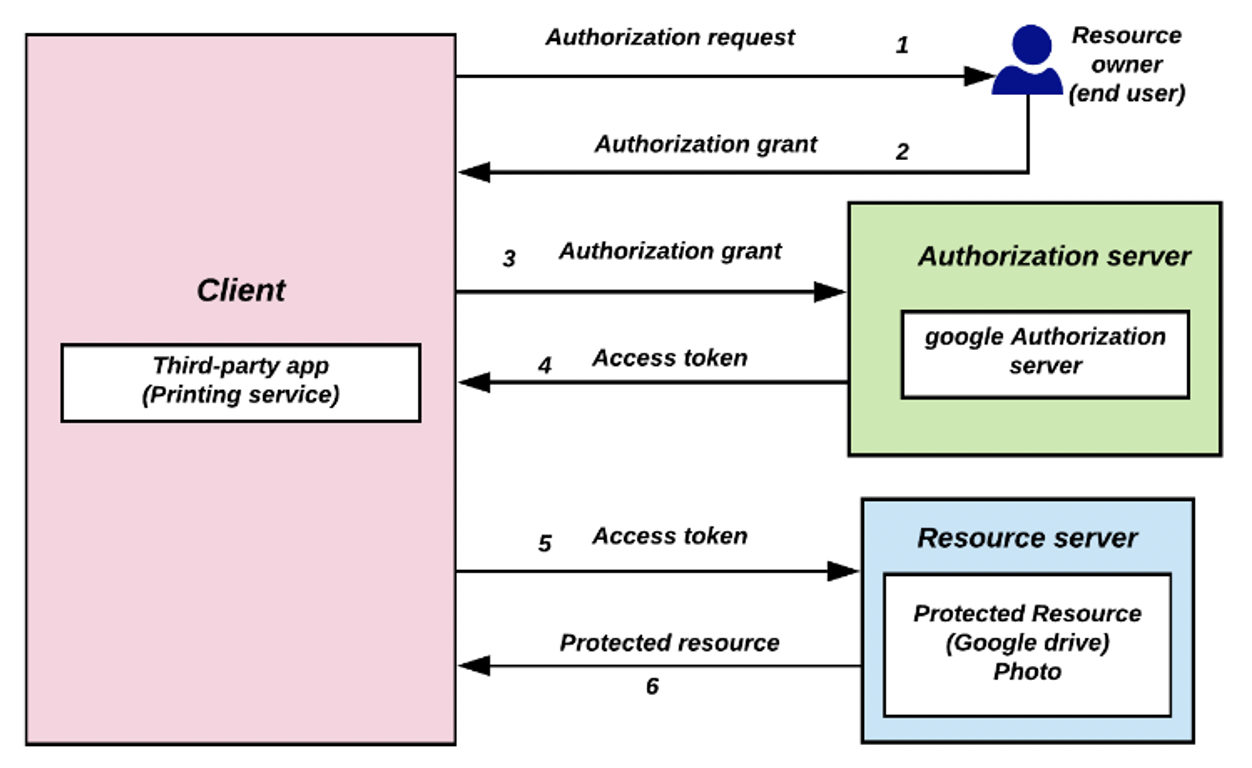
\includegraphics[width=0.75\linewidth]{oauth}
\end{center}

\prob{4} \\ In the figure showing the steps of the OAuth protocol above, at which step is
authorization to perform specific actions for different ``scopes'' (e.g., read
a file, write a file) granted? (Select the best answer.) \\
\answercircle{1}\\
\correctanswercircle{2}\\
\answercircle{3}\\
\answercircle{4}\\
\answercircle{5}
\eprob

\section*{Denial of Service Attacks}

\prob{4}  Which of the following is an example of amplification? (Select all
that apply.)\\
\correctanswercircle{A small DNS query elicits a large DNS response.} \\
\answercircle{A large number of packets is sent to a single IP address.} \\
\correctanswercircle{A ``ping'' to a broadcast address results in many reply messages.} \\
\answercircle{A large number of packets is sent to a single port.} \\
\eprob

\prob{2}  Traffic from legitimate users can exacerbate the effects of a denial of
service attack by adding to the overall attack traffic volume. \\
\yesnoyes
\eprob


\pagebreak
\section*{Public Key Infrastructure}

\prob{4}
Suppose a web server's private key is compromised (as happened with the
Heartbleed attack that we discussed in class). Which of the following
statements is true about the incident? (Select all that apply.)\\
\correctanswercircle{The attacker may be able to decrypt all past and future messages sent to the
server.}\\
\answercircle{Using the private key, an attacker can impersonate clients to the server.}\\
\correctanswercircle{Using the private key, an attacker can impersonate the server to clients.}\\
\correctanswercircle{The server must revoke its certificate.}\\
\answercircle{All of the above}
\eprob

\prob{4}  Describe one possible attack scenario that could occur if a server relies on a
self-signed certificate and the client chooses to accept that certificate.\\
\answerbox{1}{}
\eprob

\section*{DNS Security and Privacy}

\begin{center}
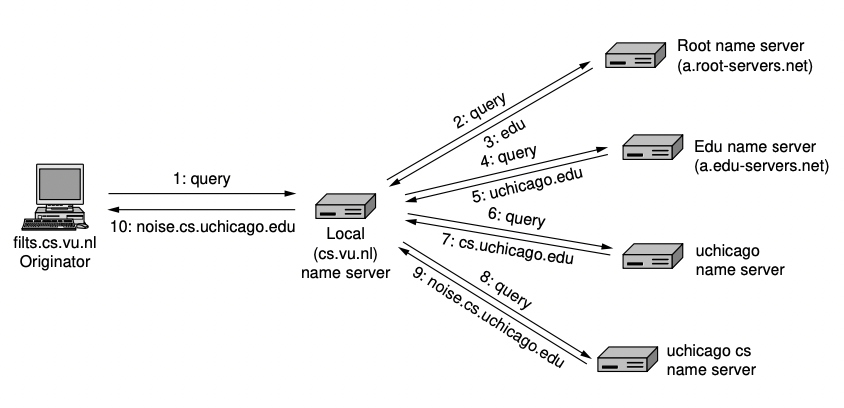
\includegraphics[width=0.75\linewidth]{dns}
\end{center}

\prob{4} 
In the above figure, circle the portion of the DNS lookup process that is
vulnerable to eavesdropping from an Internet service provider that encrypted
DNS protects against.
\eprob

\prob{2}
When encrypted DNS is enabled in your browser, the operator of the local DNS
resolver can no longer see the domain names that you are visiting.\\
\yesnono
\eprob

\pagebreak
\prob{4}
Supposing DNSSEC is widely deployed. Which of the steps in the above
transaction would contain a public key for {\tt a.edu-servers.net}? (Select
the best answer.)\\
\answercircle{2}\\
\correctanswercircle{3}\\
\answercircle{4}\\
\answercircle{6}\\
\answercircle{7}\\
\eprob

\section*{Privacy and Tracking}

\prob{4} 
Which of the following attributes can enable a user to be tracked across
websites, even in the absence of cookies? (Select all that apply.)\\
\answercircle{Installed fonts}\\
\answercircle{Browser version}\\
\answercircle{Support for gzip compression}\\
\answercircle{Type of graphics card}\\
\correctanswercircle{All of the above}\\
\eprob

\prob{4} Can the set of DNS lookups that a browser issues make it possible to determine
the specific webpage (not just the website) that a user is visiting?
\yesnoyes
\eprob

\prob{4}
Why or why not? \\
\answerbox{2.5}{}
\eprob

\pagebreak
\section*{Feedback}
\vspace*{-0.1in}
\prob{1}
Interest (1=Boring!; 10=Amazing!):
\shortanswerbox{0.5}{5}
Difficulty (1=Too easy; 10=Too hard):
\shortanswerbox{0.5}{5}
\eprob
\prob{1}
1. One thing you like. 2. One suggestion for improvement:

\answerbox{0.75}{More free food.}
\eprob

